% ##################################################################################################################
\section{Seattle Region}
\label{sec:seattle}
\hfill \textbf{Author:} Kai Nagel

\editdone{This text has undergone the professional edit. Please no grammatical changes anymore! They are most-probably wrong.}

% ##################################################################################################################
A \gls{matsim} model of the Seattle region---more precisely the \gls{psrc} area---was developed during K.\ Nagel's sabbatical stay with the \gls{urbansim} team in Seattle in 2008. The model resulted from a prototypical integration of the \gls{urbansim} software \citep[e.g.,][]{WaddellEtc2003UrbanSim} with \gls{matsim}. 

The base was an existing \gls{psrc} \gls{urbansim} model, which used an established \gls{emme2} model 
%\kai{citation!} \ah{Etwa so? \citep[][]{RolleEtAl_ITE_2007, EMME_Webpage_2008}} \kai{Ja danke.  ausser dass ich das Rolle paper nicht kenne; hoffe, es geht über emme :-)} 
as a travel model. The investigation centered around how difficult it would be to replace the \gls{emme2} model with \gls{matsim}. 

The network was taken, by conversion, from the existing \gls{emme} network, resulting in 15\,478\,links and 5\,025\,nodes with attributes length, free speed, and capacity.

Demand was generated as output from \gls{urbansim}. Evidently, the \gls{urbansim} simulation already contained a full synthetic area population. The \gls{urbansim} model was also set up with workplace choice, so that each synthetic person with ``working'' status had a workplace assigned. Since that version of \gls{urbansim} worked on the parcel level, this meant that home-to-work trips could be extracted directly, with coordinates, from the model. As so often for initial \gls{matsim}  studies, this home-to-work demand was developed into home-work-home plans.

The configuration used standard \gls{matsim} scoring parameters: a 7\,am, workplace opening time and latest work start time of 9\,am. The iterations were run with re-routing and time mutation enabled until convergence. Since this was an exercise in rapid prototyping, only a 1\,\% sample of the full synthetic population was used; road network flow and storage capacities were scaled down accordingly. Figure~\ref{fig:seattle-snapshot.left} shows a result. Figure~\ref{fig:seattle-snapshot.right} shows households most affected by a hypothetical closure of the Alaskan Way viaduct, which bypasses the Seattle downtown area, on the waterfront side to the west.
%
\createfigure%
{Seattle region scenario}%
{Seattle region scenario}%
{\label{fig:seattle-snapshot}}%
{%
  \createsubfigure%
  {Simulated congestion patterns in Seattle at 7:30\,am}%
  {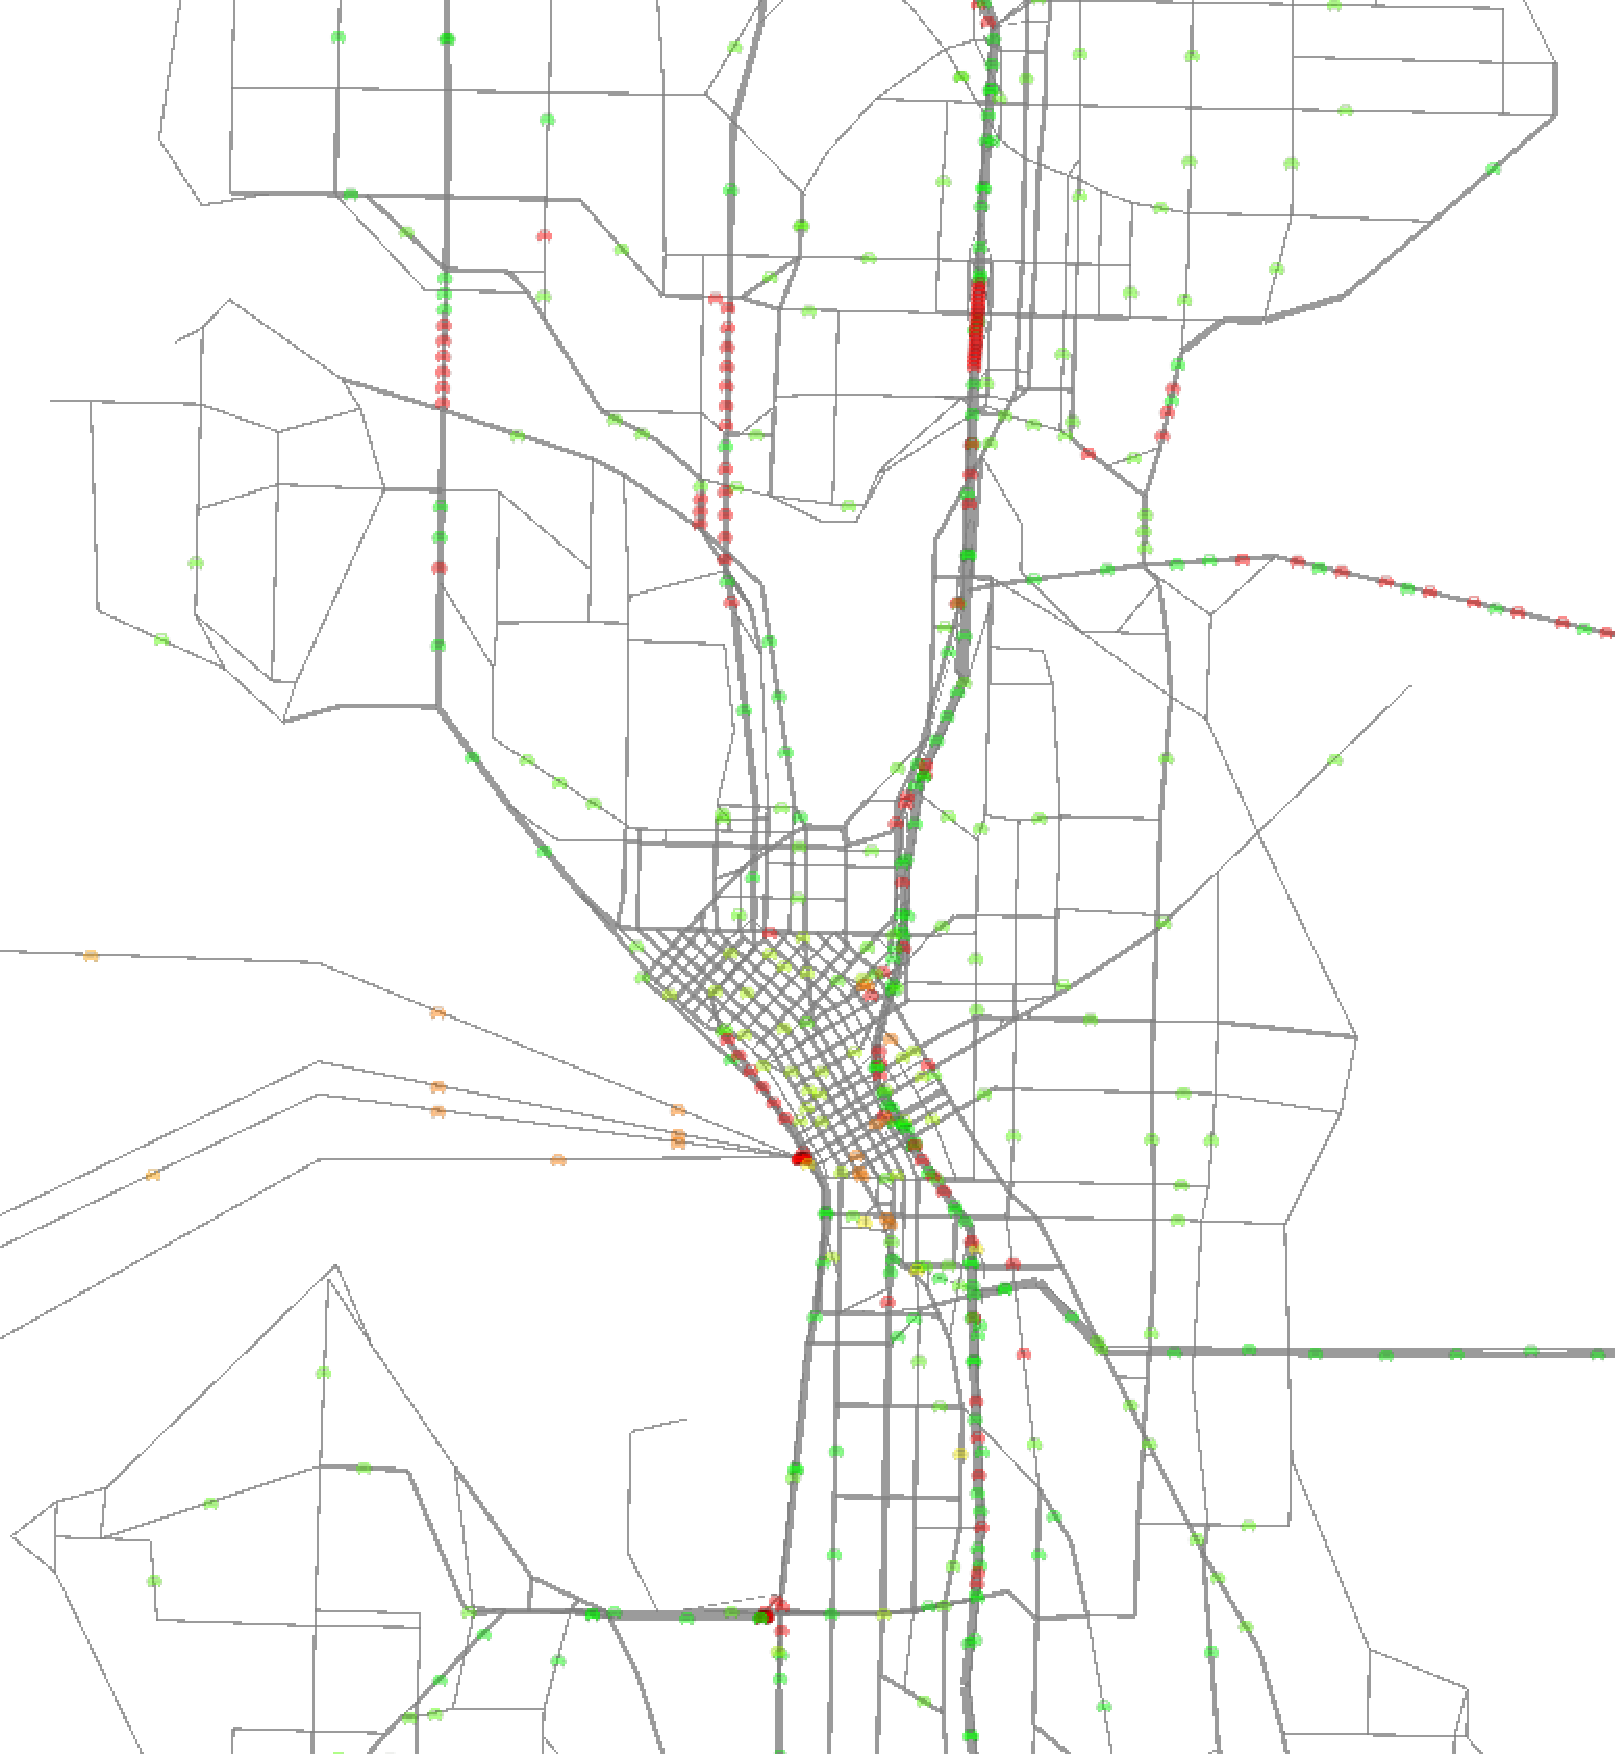
\includegraphics[width=0.49\textwidth,angle=0]{using/figures/seattle-snapshot-7h30.pdf}}%
  {\label{fig:seattle-snapshot.left}}%
  {}%
  \createsubfigure%
  {10\,\% households most affected by closure of the so-called Alaskan Way Viaduct (in red)}%
	{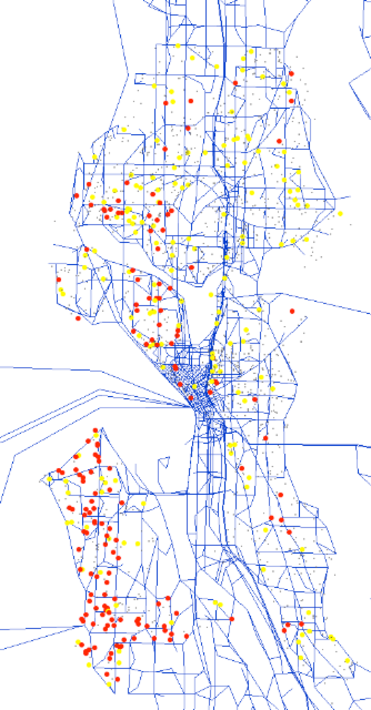
\includegraphics[width=0.49\textwidth,angle=0]{using/figures/seattle-top-10pct-0it.pdf}}%
  {\label{fig:seattle-snapshot.right}}%
  {}%
}%
{}

% ##################################################################################################################


% Local Variables:
% mode: latex
% mode: reftex
% mode: visual-line
% TeX-master: "../../main"
% comment-padding: 1
% fill-column: 9999
% End: 
